\chapter{Herramientas utilizadas}\label{cap.herramientas}
En este capítulo se van a explicar las diferentes bibliotecas software y entornos que se van a emplear, así como los lenguajes de programación de los que haremos uso.

Como lenguajes de programación se ha hecho uso de \textit{Python} y \textit{C++}. La aplicación se ha desarrollado casi en su totalidad en \textit{C++}, Aunque la integración de \textit{TensorFlow} y \textit{Keras} se ha realizado con la versión 2.7.12 de \textit{Python}.
Para el desarrollo del modelo de \textit{Deep Learning} que se empleará para la detección, se han realizado pruebas con \textit{TensorFlow}, \textit{Keras} y \textit{Darknet}. \textit{OpenCV} se ha usado para todo lo relacionado con el tratamiento de imágenes. Finalmente la evaluación experimental de la eficacia de la aplicación desarrollada se ha realizado con la herramienta \textit{DetectionSuite}.

La interfaz gráfica de la aplicación desarrollada se ha hecho con \textit{gtkmm} en \textit{C++}, herramienta que permite crear interfaces de usuario con múltiples funcionalidades.



\section{DetectionSuite}
En este proyecto se ha hecho uso de la herramienta \textit{DetectionSuite}~\cite{detectionsuite} para evaluar los resultados de las redes neuronales entrenadas y de nuestra aplicación de monitorización visual de tráfico rodado.

\textit{DetectionSuite} es una herramienta que permite evaluar diferentes tipos de redes neuronales sobre un conjunto de datos. La idea es ofrecer una infraestructura genérica para evaluar los algoritmos de detección de objetos contra un conjunto de datos estandarizado y calcular las estadísticas más comunes:
\begin{itemize}
    \item \textit{\acrfull{iou}}
    \item Precisión
    \item \textit{Recall}
\end{itemize}

La \textit{\acrfull{iou}} en la detección de objetos mide la precisión de un detector en un conjunto de datos en particular y sigue la siguiente fórmula:

\begin{equation}\label{iou}
IoU = \frac{AreaofOverlap}{AreaofUnion}
\end{equation}

Donde \textit{AreaofOverlap} es el área que pertenece a la intersección entre la predicción y la realidad, mientras que \textit{AreaofUnion} es el área suma (sin repetición del solape) de la predicción y la realidad según muestra la Figura \ref{fig.formula_iou}.

En la Figura \ref{fig.ejemplo_iou} se puede ver un ejemplo visual del \textit{ground-truth} y la predicción obtenida. En este caso el \textit{AreaofOverlap} es el área que incluye únicamente la intersección entre lo que hemos predecido y el \textit{ground-truth}. Y el \textit{AreaofUnion} es el área que se forma entre el \textit{ground-truth} y la predicción.

\begin{figure}[H]
  \begin{center}
    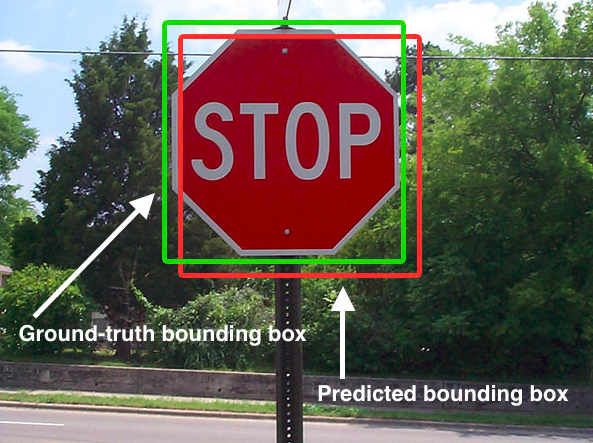
\includegraphics[width=0.6\textwidth]{figures/Herramientas/iou.png}
		\caption{Ejemplo de \acrshort{iou}}
		\label{fig.ejemplo_iou}
		\end{center}
\end{figure}


\begin{figure}[H]
  \begin{center}
    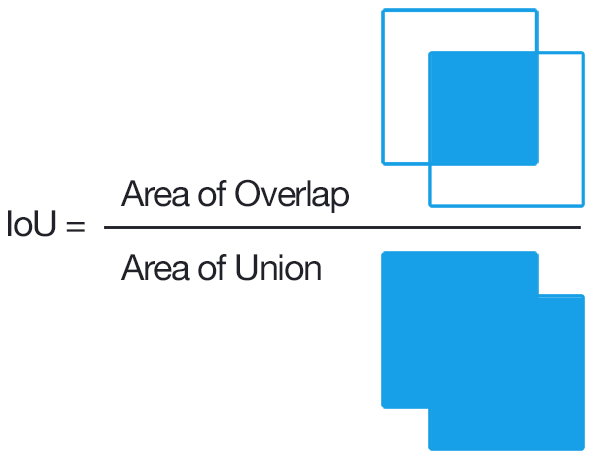
\includegraphics[width=0.4\textwidth]{figures/Herramientas/iou_formula.png}
		\caption{Fórmula \acrshort{iou}}
		\label{fig.formula_iou}
		\end{center}
\end{figure}

Antes de explicar la precisión y el \textit{recall} hay que aclarar algunos términos empleados a la hora de evaluar los resultados de las detecciones. 

\begin{itemize}
    \item \textit{True Positive (TP)}: son los verdaderos positivos, es decir aquellas detecciones que se han hecho correctamente.
    \item \textit{False Positive (FP)}: falsos positivos. Son aquellas detecciones que se han hecho pero son erróneas.
    \item \textit{False Negative (FN)}: falsos negativos. Es la proporción de casos positivos que la prueba detecta como negativos, es decir objetos que no se han detectado y deberían haberse detectado.
    \item \textit{True Negative (TN)}: verdadero negativo. Se refiere a los \textit{boundingbox} que no deben detectarse en la imagen y no se han detectado. Este valor no se emplea en las métricas.
\end{itemize}

La precisión se trata del total de detecciones correctas entre la cantidad de detecciones obtenidas. La precisión que obtiene \textit{DetectionSuite} es la promediada (\textit{\acrfull{map}}), para aquellas predicciones que tienen un \acrshort{iou} mayor que un umbral (0.5).

\begin{equation}\label{precision}
Precision = \frac{TP}{TP + FP}
\end{equation}

El \textit{recall} es la cantidad de detecciones correctas entre la cantidad de detecciones reales, es decir las detecciones del \textit{ground-truth}. Al igual que la precisión, se obtiene un promediado (\textit{\acrfull{mar}}) de las detecciones que tienen un \acrshort{iou} superior a 0.5.

\begin{equation}\label{recall}
Precision = \frac{TP}{TP + FN}
\end{equation}

Volviendo a \textit{DetectionSuite}, es una herramienta que puede emplearse tanto en Linux como en MacOS. Permite evaluar modelos entrenados en \textit{Tensorflow}, \textit{Keras}, \textit{Caffe} y \textit{Darknet}. Los formatos de dataset que admite son:  \acrshort{yolo}, \acrshort{coco}, \textit{ImageNet Pascal VOC}, etc. A continuación se enumeran las entradas de imágenes soportadas:

\begin{itemize}
    \item WebCamera/ USB Camera
    \item Vídeos
    \item Streams from ROS
    \item Streams from ICE
    \item JdeRobot Recorder Logs
\end{itemize}

En este \acrshort{tfm} en concreto se va a hacer uso de la herramienta \textit{AutoEvaluator} de \textit{DetectionSuite}, la cual es capaz de evaluar múltiples redes en un solo conjunto de datos o múltiples conjuntos de datos en una sola ejecución. Todo lo que necesita es un archivo de configuración que contenga detalles sobre los conjuntos de datos y las redes. Los resultados se escriben en archivos CSV en el directorio de salida especificado.

\section{Entorno TensorFlow}
Para el desarrollo de la red neuronal que queremos aplicar en nuestra aplicación \textit{Smart-Traffic-Sensor} se  han probado diferentes plataformas de desarrollo de \textit{Deep Learning}, entre ellas \textit{TensorFlow} \footnote{https://www.tensorflow.org/}. Es una plataforma de código abierto \textit{end-to-end} para el \textit{Machine Learning} que fue liberada bajo licencia de \textit{Apache} 2 a finales de 2015 y que está disponible en github~\cite{github_tensorflow}. Fue desarrollada por el equipo de investigación en \textit{Machine Learning “Google Brain”}  en \textit{C++} y \textit{Python}, y es usado en multitud de productos y servicios de Google como Gmail o \textit{Google Translation}. Google ofrece en su plataforma \textit{Cloud} ejecutar \textit{Tensorflow} en \textit{Tensor Processing Unit} (TPU), un nuevo tipo de procesadores en \textit{Cloud} optimizados para ejecutar \acrfull{ia}.  \textit{TensorFlow} está orientado a problemas de \textit{Deep Learning} y permite entrenar y construir redes neuronales. 

\textit{TensorFlow} puede correr tanto en CPUs como en GPUs (haciendo uso de \acrfull{cuda}). Está disponible en \textit{Linux} de 64 bits, \textit{MacOS}, y plataformas móviles que incluyen \textit{Android} e \textit{iOS}. Actualmente es el entorno más popular en \textit{Deep Learning}.

Puede ejecutar de forma rápida y eficiente gráficos de flujo. Un gráfico de flujo está formado por operaciones matemáticas representadas sobre nodos, y cuya entrada y salida es un vector multidimensional o tensor de datos, por este motivo recibe el nombre de \textit{TensorFlow}.

Las ventajas de este software se extienden a muchas disciplinas a parte de la tecnología TIC. Se emplea en medicina en imágenes médicas para la detección de tumores por ejemplo, también se usa en la detección y combinación de estilos artísticos en la pintura, etc.

En este \acrshort{tfm} se emplea la versión 1.12.0 de \textit{Tensorflow}.

\section{Entorno Keras}

Al igual que se ha empleado \textit{TensorFlow} como plataforma de desarrollo de la red neuronal, se ha hecho uso de \textit{Keras} \footnote{https://keras.io/}. Es un entorno de alto nivel para el aprendizaje, escrito en \textit{Python} y capaz de correr sobre \textit{TensorFlow}, \acrshort{cntk}, o \textit{Theano}. Fue desarrollado con el objetivo de facilitar el proceso de experimentación en redes neuronales de forma rápida y eficiente. Puede correr tanto en CPU como en GPU. Permite crear de forma sencilla y rápida los modelos de las redes neuronales (a través de su facilidad de uso, su modularidad y su extensibilidad). Admite redes convolucionales y redes recurrentes, así como combinaciones de las dos.

Inicialmente fue desarrollada en el proyecto de investigación ONEIROS (Open--ended Neuro--Electronic Intelligent Robot Operating System). Su creador es Fran\c{c}ois Chollet, ingeniero de \textit{Google}.
En 2017, el equipo de TensorFlow de Google decidió dar soporte a Keras en la biblioteca de core de TensorFlow.

Al igual que \textit{TensorFlow}, \textit{Keras} se encuentra en github~\cite{keras_github}, pues es de código abierto. 

Las principales ventajas de \textit{Keras} son que es fácil de usar, modular, y relativamente fácil de extender, haciendo muy simple su uso. Con \textit{Keras} puedes realizar redes neuronales de forma sencilla y con muy pocas líneas de código, a diferencia de \textit{TensorFlow} que es algo más complejo. 

En este proyecto se hace uso de la versión 2.2.4 de \textit{Keras}.


\section{Entorno Darknet}

\textit{Darknet} \footnote{https://pjreddie.com/darknet/} es un entorno para redes neuronales de código abierto escrito en C y \acrshort{cuda}. Es rápido, fácil de instalar y admite el empleo de CPU y GPU. El código se puede encontrar en github~\cite{darknet_github}.

\textit{Darknet} se creó con el fin de emplearse en el diseño, ejecución y entrenamiento de redes neuronales profundas para la clasificación y detección de objetos. Las principales ventajas de este sistema son su simplicidad en términos de uso y su tama\~{n}o reducido.

En nuestro proyecto haremos uso de \acrfull{yolo}, que es un sistema de detección de objetos que funciona sobre \textit{Darknet}. \acrshort{yolo} utiliza \textit{Deep Learning} y \acrshort{cnn} para detectar objetos, y se distingue de sus competidores porque requiere de ver la imagen una sola vez, permitiéndole ser mucho más rápido que el resto de algoritmos. Gracias a su gran rapidez es capaz de detectar objetos en tiempo real en vídeos (hasta 30 \textit{\acrshort{fps}}).

A la hora de realizar la detección, \acrshort{yolo} en primer lugar divide la imagen en una cuadrícula de SxS. En cada una de sus celdas se estiman sus N posibles \textit{bounding boxes}  con sus respectivas probabilidades de acierto. Teniendo así SxSxN \textit{bounding boxes}. Aquellas predicciones que tengan una probabilidad por debajo de un umbral quedarán eliminadas. A las que superen dicho umbral se les aplicará \textit{non--max suppression}, lo cual sirve para eliminar objetos detectados por duplicado. Este proceso puede verse en la  Figura \ref{fig.yolo}.

\begin{figure}[H]
  \begin{center}
    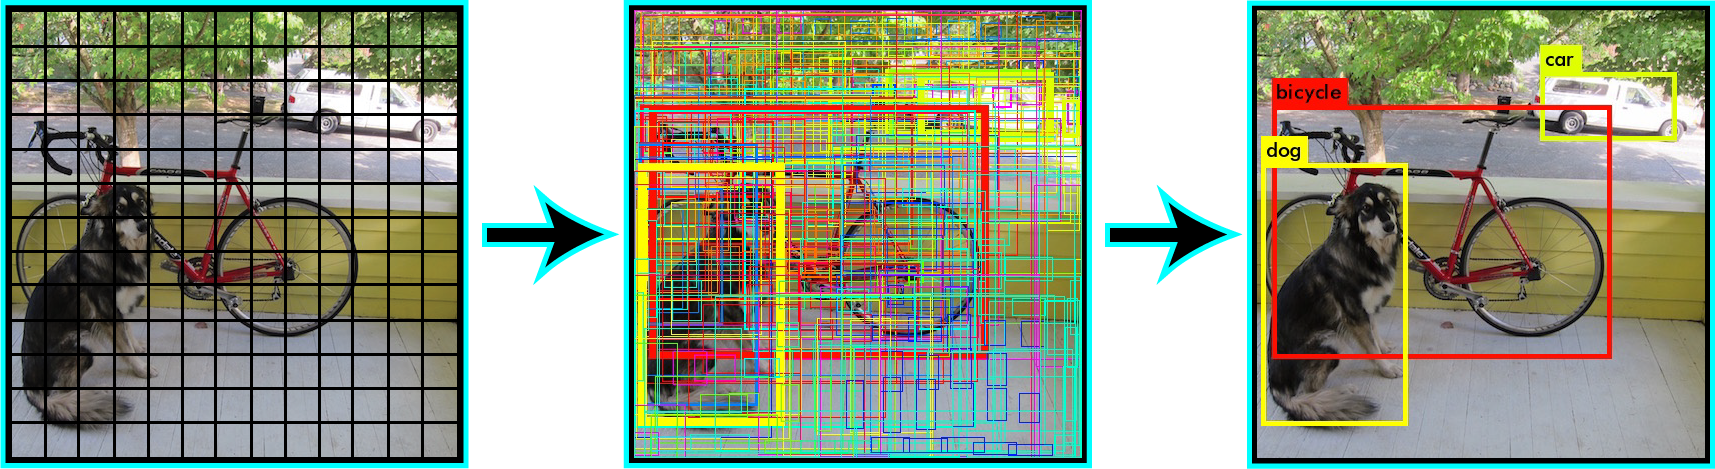
\includegraphics[width=0.9\textwidth]{figures/Herramientas/yolo.png}
		\caption{Proceso de Yolo}
		\label{fig.yolo}
		\end{center}
\end{figure}

En este \acrshort{tfm} se ha usado \textit{Darknet} para el desarrollo de una red neuronal. La versión que se ha empleado es \textit{YOLOv3}, es decir, la última versión existente hasta la fecha.

\section{Biblioteca OpenCV}

\textit{OpenCV} \footnote{https://opencv.org/} es una librería de código abierto desarrollada por \textit{Intel} y publicada  bajo licenciade BSD. Esta librería implementa gran variedad de herramientas para la interpretación de la imagen. Sus  siglas  provienen  de  los  términos anglosajones ``\textit{Open Source Computer  Vision Library}", y tal y como se puede deducir es una librería destinada a aplicaciones de visión por computador en tiempo real. Puede ser empleada en MacOS, Windows y Linux,y existen versiones para \textit{C\#}, \textit{Python} y \textit{Java}, a pesar de que originalmente era una librería en \textit{C/C++}. Además hay interfaces para \textit{Ruby}, \textit{Python}, \textit{Matlab} y otros lenguajes. 

\textit{OpenCV} implementa algoritmos para técnicas de calibración, detección de rasgos, rastreo, análisis de la forma, análisis del movimiento, reconstrucción 3D, segmentación de objetos y reconocimiento, etc. Los algoritmos se basan  en  estructuras de datos flexibles acopladas con estructuras IPL (\textit{Intel  Image Processing Library}), aprovechándose de la arquitectura de Intel en la optimización de más de las mitad de las funciones. Incorpora funciones básicas para modelar el fondo, sustraer dicho  fondo y generar imágenes de movimiento MHI  (\textit{Motion  History  Images}).  Además  incluye  funciones para determinar dónde hubo movimiento y en qué dirección. 

\begin{figure}[H]
  \begin{center}
    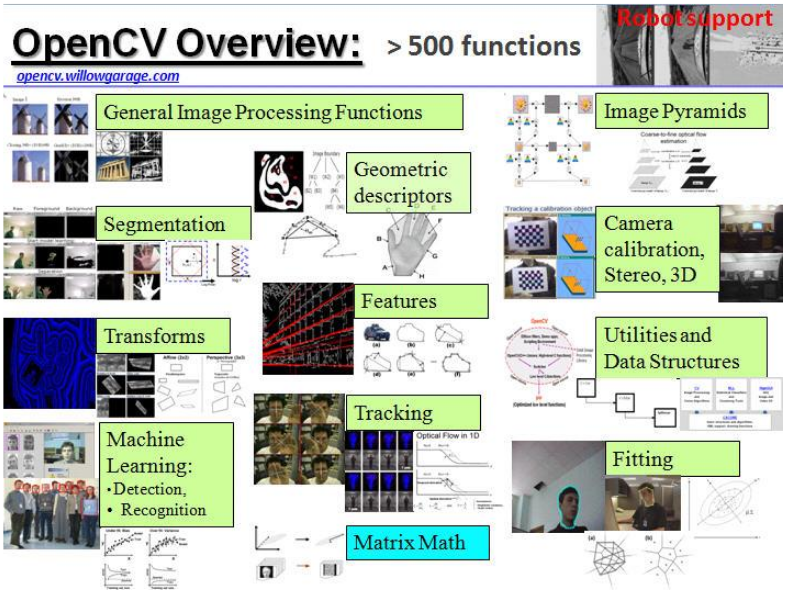
\includegraphics[width=0.6\textwidth]{figures/Herramientas/opencv.png}
		\caption{Funciones de OpenCV}
		\label{fig.opencv}
		\end{center}
\end{figure}

Fue diseñado para tener una alta eficiencia computacional, está escrito en C y puede aprovechar las ventajas de los procesadores multinúcleo. Contiene más  de  2500  funciones  que  abarcan  muchas  áreas  de  la  visión  artificial.  También  tiene  una librería   de   aprendizaje   automático   (MLL,  \textit{Machine   Learning   Library})   destinada   al reconocimiento  y agrupación de patrones estadísticos.

Desde su aparición OpenCV ha sido usado en numerosas aplicaciones. Entre las cuales se encuentran la unión de imágenes de satélites y mapas web, la reducción de ruido en imágenes  médicas,  los  sistemas  de  detección  de movimiento,  la  calibración  de  cámaras,  el manejo  de  vehículos  no  tripulados, el  reconocimiento  de  gestos, etc. OpenCV  es  empleado también  en  reconocimiento  de  música  y  sonido,  mediante  la  aplicación  de  técnicas  de reconocimiento de visión en imágenes de espectrogramas del sonido.

Hay  una  gran  cantidad  de  empresas    y  centros  de  investigación  que  emplean  estas técnicas como IBM, Microsoft, Intel, SONY, Siemens, Google, Stanford, MIT, CMU, Cambridge e INRIA.

En este proyecto se hace uso de la versión \textit{OpenCV} 3.2.


\section{Biblioteca Gtkmm}

\textit{Gtkmm} \footnote{http://www.gtkmm.org} es una encapsulación en \textit{C++} de \textit{Gtk+}. Dicha encapsulación ofrece todos los beneficios de la orientación a objetos, e incorpora otras cualidades como una mejora en la comprobación de tipos, código más reducido y legible, y un menor uso de los punteros. 

Se trata de un \textit{toolkit} para desarrollar interfaces gráficas de usuario. Es un software libre distribuido bajo la Licencia Pública General Reducida de GNU (LGPL).

\textit{Gtkmm} se organiza por medio de ventanas, las cuales contienen \textit{widgets}, como por ejemplo botones etiquetas, cuadros de texto, etc.  Para cada \textit{widget} debemos tener un objeto C++ con el cual controlar su funcionamiento, es decir si por ejemplo nuestro \textit{widget} es un botón, necesitaremos funciones para saber si se ha pulsado o no, y acerca de que realizar si se hubiera pulsado, para todo ello se emplea un objeto de C++. 

Aunque se puede especificar el diseño y apariencia de las ventanas y \textit{widgets} con C++, resulta más conveniente usar \textit{Glade} para el diseño de la interfaz de usuario y cargarlos en tiempo de ejecución con \textit{Gtk::Builder}. Con  \textit{Glade} podemos desarrollar las interfaces de usuario, guardarlas en formato .glade y luego cargarlas desde \textit{gtkmm} empleando \textit{ Gtk::Builder}.

En este caso se hace uso de la versión \textit{gtkmm} 3.0.



